\noindent In overview, thus far we have take a progression of reasonable, small steps to building a relativistic quantum field theory. We established Lorentz invariance as a symmetry of the theory, which may not quite be a fundamental symmetry of nature, but has not been violated by any experiments to date. Next, we established a unitary representation of the Poincar\'e group (difficult since the Poincar\'e group is not compact, unlike rotation groups), where space and time can transform into other via Lorentz boosts, meaning that energy and momentum can also exchange roles under Poincar\'e symmetries. This also causes difficulties in writing down quantum mechanical Hamiltonians that behave appropriately, but, fortunately, we can invoke locality in the theory, which is also seemingly fundamental to nature. Motivated by classical examples, such as the Klein-Gordon equation, a free theory, we write the relativistic quantum field theory, namely the quantum Klein-Gordon field, by "just putting hats" on the operators, and it worked. \\

\noindent To account for interactions, we added a perturbative $\varphi^4$ term to the quantum Klein-Gordon Hamiltonian
\begin{equation}
\hat{H}_{KG} \to \hat{H}_{KG} + \hat{H}_{\varphi^4}
\end{equation}

\noindent Where $\hat{H}_{\varphi^4}$ is Lorentz invariant, but is also an unbounded operator on any Hilbert space, such that $||\hat{H}_{\varphi^4} || \to \infty$. Though this is not mathematically rigorous, our forefathers and foremothers have shown through physical rigor, as well as time and time again by using tools outside of the realm of their mathematical applicability, that this is an acceptable perturbative term to account for field interactions. \\

\subsection*{Examples of Mathematically Non-Rigorous Applications}

\begin{itemize}
\item The building block of perturbation theory assumes that the interacting theory vacuum state is proportional to the free theory vacuum state via the time-evolution operator of the interacting theory
	\subitem $\ket{\Omega} \propto \lim_{t\to\infty} e^{-i\hat{H}_{\varphi^4}t} \ket{\Omega_0}$.
	\begin{itemize} 
	\item Even for finite dimensional systems, this limit does not exist and is oscillatory. The limit can make sense for Hamiltonians with a continuous spectra with a few particles.
	\end{itemize}
\item The momentum eigenstates require preparation of delta functions in the momenta, and are assumed to be related similar to the vacuum states
	\subitem $\ket{\textbf{p}_1 \dots \textbf{p}_n} = \lim_{t\to\infty} e^{-i\hat{H}_{\varphi^4}t} \ket{\textbf{p}_1 \dots \textbf{p}_n}_0$.
\item The Dyson series, a Taylor expansion of the interacting theory time evolution operator can not be expected to converge
	\subitem $e^{-i\hat{H}_{\varphi^4}t} = e^{-i\hat{H}_{KG}t} -i \int_0^t dt' \, e^{-i\hat{H}_{KG}t'} \hat{H}_I e^{i\hat{H}_{KG}t'} + \dots$.
\end{itemize}

\noindent We are often punished by infinities, where we would prefer finite numbers. Some infinities are trivially removable with no operational consequence, such as the ground state energy shift in the Klein-Gordon theory, such that $E_0 \to E_0 + \infty$ . Other infinities can be factored away by rescaling observables, such as in the case of vacuum bubbles (e.g., $\frac{\infty}{\infty} = 1$). Yet other infinities just don't go away, such as in the diagram of two internal vertices. \\

\noindent Perhaps the choice of interaction terms is the cause of all of these infinities, and we can impose a cutoff to the theory that will eliminate some infinities. For example, in the $\varphi^4$ theory
\begin{equation}
\hat{H}_{\varphi^4} \to \hat{H}_{\varphi^4}(\Lambda)
\end{equation}

\noindent Where $\Lambda$ is a cutoff up to some family of models/theories, and the norm of the cutoff Hamiltonian is proportional to the cutoff, which may be large, but not infinity, such that $||\hat{H}_{\varphi^4}(\Lambda) || \propto \Lambda$. \\

\noindent For example, consider the quantum harmonic oscillator cutoff, where $||\hat{H}(N)|| = N$
\begin{equation}
\hat{H} = \sum_{n=0}^{\infty} (n+\frac{1}{2}) \ket{n}\bra{n} \to \hat{H}(N) = \sum_{n=0}^N (n+\frac{1}{2}) \ket{n}\bra{n} + \sum_{n>N} (N+\frac{1}{2}) \ket{n}\bra{n}
\end{equation}

\noindent The major concern with imposing cutoffs is whether observables depend on the cutoff or not. To eschew this issue, we allow unobservable parameters, coupling constants, to shift and absorb all the cutoff dependence. \\

\subsection*{Renormalization}

\noindent This practice is called \textbf{renormalization}, and it works. We make the hypothesis that the Hamiltonian depends on some number of parameters, called coupling constants, such that $\hat{H} = \hat{H}(z_1,\dots,z_n)$. The mapping from the coupling constants to observables is not expected to be, and is usually not, bijective. For example,
\begin{equation}
\hat{H}_{\varphi^4}(\lambda, m) = \int d^3 x \, \left( \nabla^2 \hat{\phi} + m^2 \hat{\phi}^2 + \frac{\lambda}{4!} \hat{\phi}^4 \right)
\end{equation}

\noindent This Hamiltonian corresponds to a list of observables $\mathcal{O}_j(z_1,\dots, z_n)$, $j=1,2,\dots$, with complicated (nonlinear) dependencies with the coupling constants, which usuaslly exist on a smooth manifold before mapping to observables. \\

\noindent For example, consider the spectral gap $\mathcal{O} = E_1-E_0$, where $\mathcal{O} = \mathcal{O}(z_1+c,z_2,\dots,z_n)$, and $\hat{H} = z_1\cdot \mathbb{I} + \hat{H}'(z_2,\dots,z_n)$. \\

\noindent Add the cutoff dependence to the observables, such that 
\begin{equation}
\hat{H}_\Lambda (z_1,\dots, z_n) \to \mathcal{O}_{expt.} = \mathcal{O}_j(z_1,\dots,z_n;\Lambda)
\end{equation}

\noindent If "lucky", each of the coupling constants can absorb all of the $\Lambda$-dependence, and none of the observables will depend directly on the cutoff
\begin{equation}
\mathcal{O}_{expt.} = \mathcal{O}_j(z_1,\dots,z_n;\Lambda) = \mathcal{O}_j(z_1(\Lambda) , \dots , z_n(\Lambda)) .
\end{equation}

\noindent If the above is true, then the theory is renormalizable, and is now defined by a highly overdetermined set of equations, such that there are a finite number of parameters $z_i$ and an infinite list of equations (observables) $\mathcal{O}_j$ to solve. Renormalizable theories effectively have no cutoff, since the remaining infinities are eliminated by changing the order of limits.
\begin{enumerate}
\item Take the limit as the cutoff tends to infinity, $\Lambda \to \infty$, then compute observable quantities.
\item Vice versa.
\end{enumerate}

\subsection*{Typical Terms in Scattering Experiments}

\noindent Scattering experiments generate interaction terms such as the following
\begin{equation}
\,_0 \bra{p_1 p_2 \dots p_n} \mathcal{T} \, [\frac{\lambda}{4!} \int d^4 x \, \hat{\phi}_I^4(x)]\ket{q_A q_B}_0 \,.
\end{equation}

\noindent Apply (generalized) Wick's theorem to calculate the contractions, and sum over three types of terms (to order $\lambda$) encountered. Note that $\hat{\phi}_I (x) = \hat{\phi}$ in the following. Wick's theorem applied to $\mathcal{T}[\hat{\phi}^4 (x)]$ yields a sum over the normal ordering of all of the following contractions, such that 
\begin{equation}
\mathcal{T}[\hat{\phi}^4 (x)] = \text{fully contracted} + \text{partially contracted} + \text{uncontracted}
\end{equation}
\begin{align*}
\textbf{Fully contracted}: &\,\,\,\, \mathcal{N}[ \wick[offset=1.2em]{\c1 {\hat{\phi}} \c1 {\hat{\phi}} \c2 {\hat{\phi}} \c2 {\hat{\phi}} }] + \text{other fully contracted} \\
\textbf{Partially contracted}: &\,\,\,\, \mathcal{N}[ \wick[offset=1.2em]{\c {\hat{\phi}} \c {\hat{\phi}} {\hat{\phi}} {\hat{\phi}}} + \wick[offset=1.2em]{\c {\hat{\phi}} {\hat{\phi}} \c {\hat{\phi}} {\hat{\phi}}}] + \text{other partially contracted} \\
\textbf{Uncontracted}: &\,\,\,\, \mathcal{N} [ \hat{\phi} \hat{\phi} \hat{\phi} \hat{\phi}].
\end{align*}

\noindent The diagrammatic contributions to the integrals from each type of contracted term to the $\mathcal{S}$-matrix have the following forms (for the $n=2$ case) \\

\noindent \textbf{Type 1, fully contracted:} 

\begin{equation}
\frac{-i\lambda}{4!} \int d^4 x \,_0 \bra{p_1 p_2} \wick[offset=1.2em]{\c1 {\hat{\phi}} \c1 {\hat{\phi}} \c2 {\hat{\phi}} \c2 {\hat{\phi}} } \ket{q_A q_B}_0 =
\end{equation}
\begin{figure}[H]
	\centering
	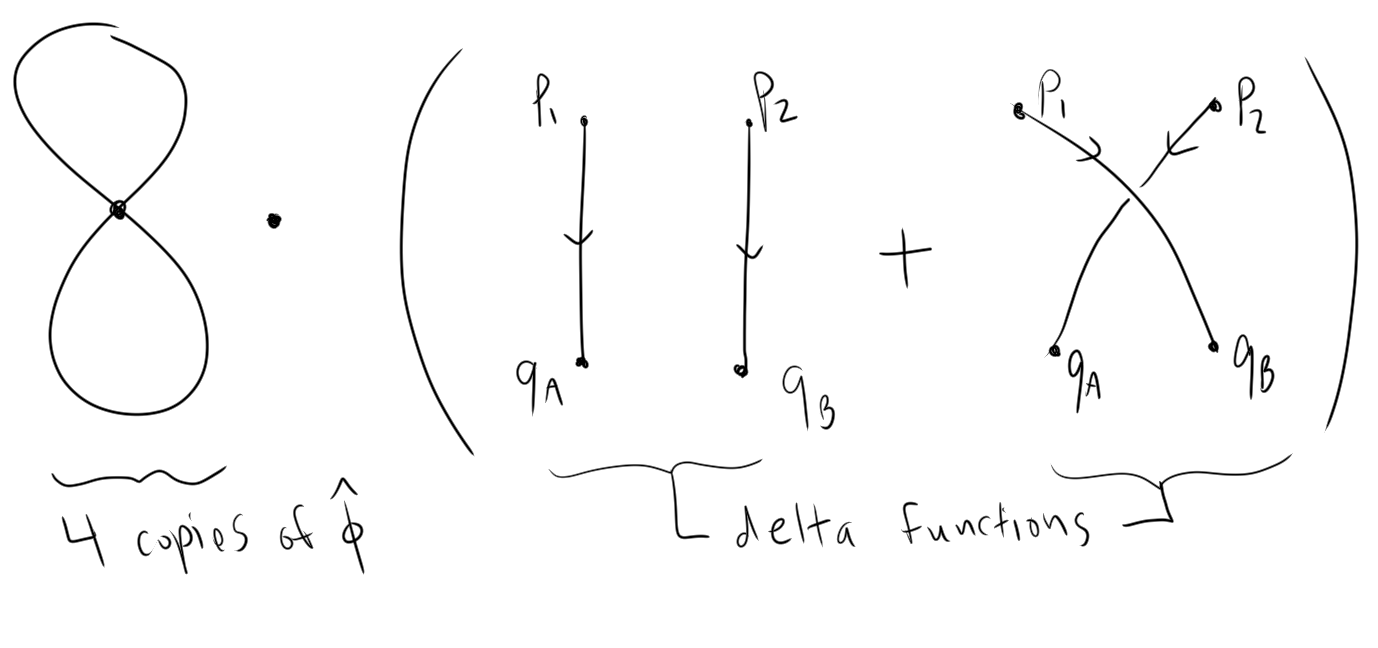
\includegraphics[scale=0.4]{images/fullcont.png}
	\caption{Diagrammatic contributions of fully contracted terms: a product of fully connected diagrams, from four copies of the field operator (figure eight), and delta functions imposing a sort of momentum conservation.}
\end{figure}

\noindent The full contraction is just a $\mathbb{C}$ number, making the integral over the inner product of momentum eigenstates. \\

\noindent \textbf{Type 2, partially contracted:}

\begin{equation}
\frac{-i\lambda}{4!} \int d^4 x \,\,_0\bra{p_1 p_2} \wick[offset=1.2em]{\c {\hat{\phi}} \c {\hat{\phi}}} \,\mathcal{N}[\hat{\phi} \hat{\phi}] \ket{q_A q_B}_0 = \frac{-i\lambda}{4!} \int d^4 x \, ( \, (1) + (2) + (3) \, )
\end{equation}

\noindent The partial contractions have three more types of normal orderings, as labelled above: $(1) + (2) + (3)$
\begin{enumerate}
\item \textbf{Right:} $\wick[offset=1.5em]{\c {\hat{\phi}} \c {\hat{\phi}}} \,\,_0\bra{p_1 p_2} \wick[offset=1.5em]{\c1 {\hat{\phi}} \c2 {\hat{\phi}} \ket{ \c1 {q_A} \c2{q_B} }_0 } + $ all other contractions to the right.
\item \textbf{Left:} $\wick[offset=1.5em]{\c {\hat{\phi}} \c {\hat{\phi}}} \, \wick[offset=1.5em]{ \,_0\bra{ \c1 {p_1} \c2 {p_2} } \c2 {\hat{\phi}} \c1 {\hat{\phi}}} \ket{q_A q_B}_0  + $ all other contractions to the left.
\item \textbf{Both:} $\wick[offset=1.5em]{\c {\hat{\phi}} \c {\hat{\phi}}} \, \wick[offset=1.5em]{ \,_0\bra{ \c1 {p_1} p_2} \c1 {\hat{\phi}} \c2 {\hat{\phi}} \ket{ \c2 {q_A} q_B }_0 } + $ all other contractions one left and one right.
\end{enumerate}

\begin{figure}[H]
	\centering
	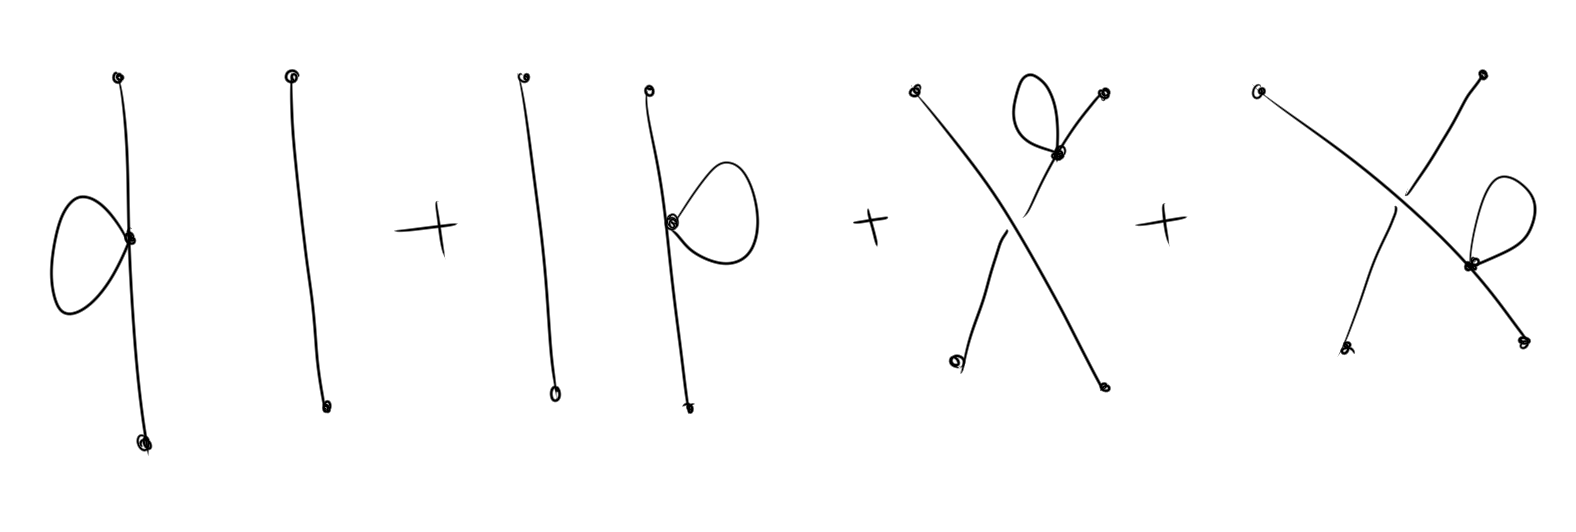
\includegraphics[scale=0.4]{images/partcont.png}
	\caption{Diagrammatic contributions of partially contracted terms.}
\end{figure}

\noindent Note that the contraction of the interacting field operators and the momentum eigenstates, as in the three cases above, contribute incoming/outgoing momenta, a vertex, and three external legs.

\begin{figure}[H]
	\centering
	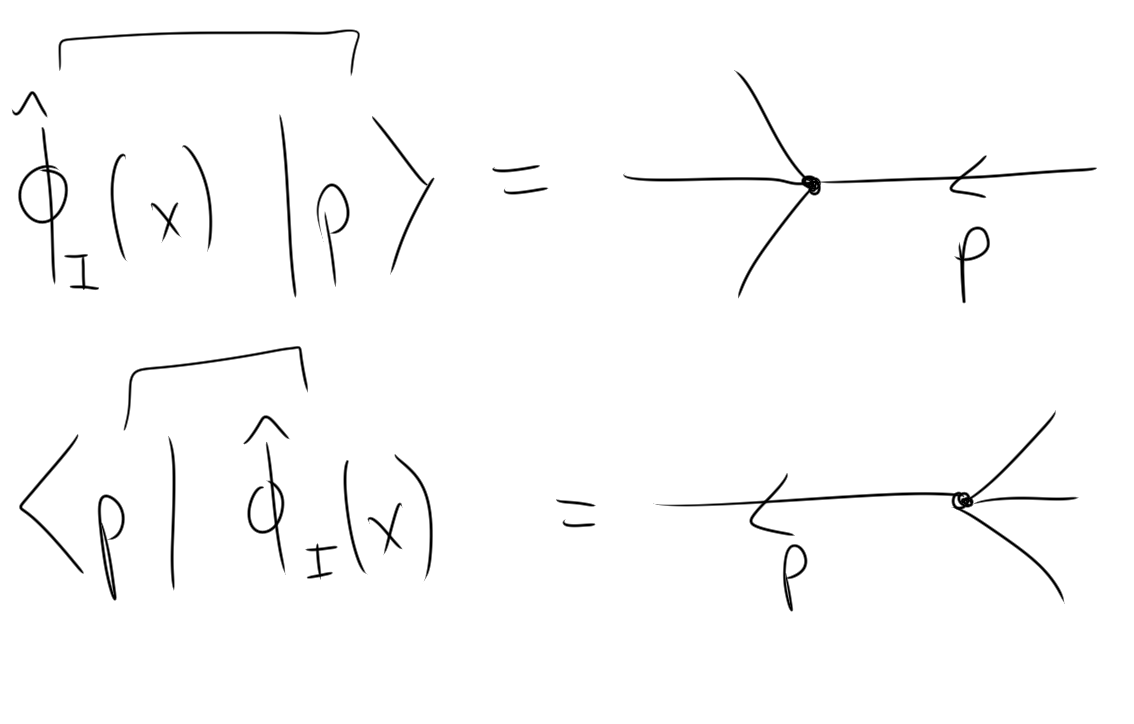
\includegraphics[scale=0.3]{images/opstatecont.png}
	\caption{Diagrammatic contributions of contractions between intertacting field operators and momentum eigenstates.}
\end{figure}

\noindent \textbf{Type 3, uncontracted:} 

\begin{align*}
\frac{-i\lambda}{4!} \int d^4 x \,\,_0\bra{p_1 p_2} \mathcal{N}[\hat{\phi} \hat{\phi} \hat{\phi} \hat{\phi}] \ket{q_A q_B}_0 &= \, \frac{-i\lambda}{4!} \cdot 4! \cdot \int d^4 x e^{-i(q_A + q_B - p_1 - p_2) \cdot x} \\
&= -i \lambda (2 \pi)^4 \delta^{(4)} (q_A + q_B - p_1 - p_2) \\
&= \text{Diagram below.}
\end{align*}

\begin{figure}[H]
	\centering
	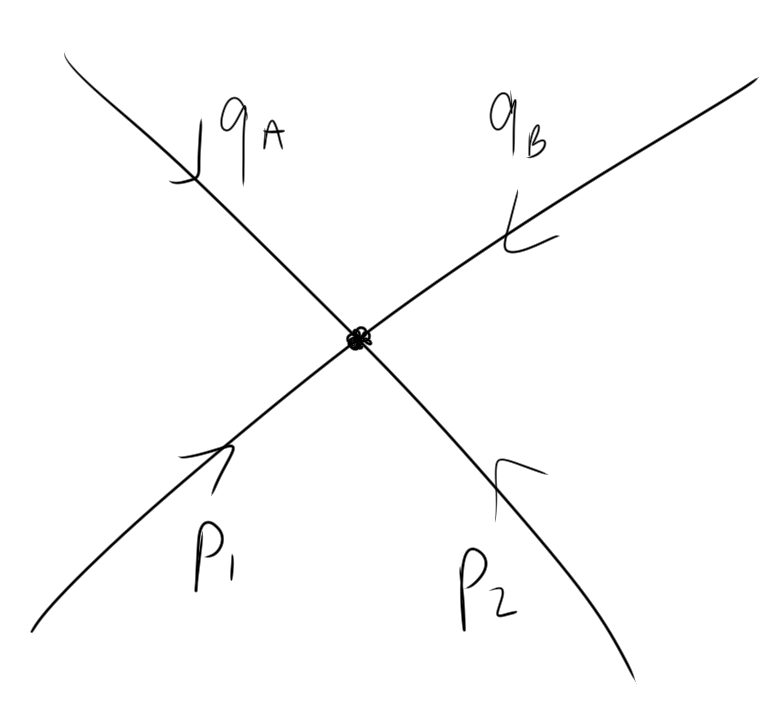
\includegraphics[scale=0.3]{images/momcons.png}
	\caption{Uncontracted term contributes diagram that enforces momentum conservation.}
\end{figure}

\noindent Adding all of the terms together in the full expansion of the interacting component of the $\mathcal{S}$-matrix, namely $\,_0\bra{p_1 p_2} i\hat{\mathbb{T}} \ket{q_A q_B}_0$, we get a series lke the following

\begin{figure}[H]
	\centering
	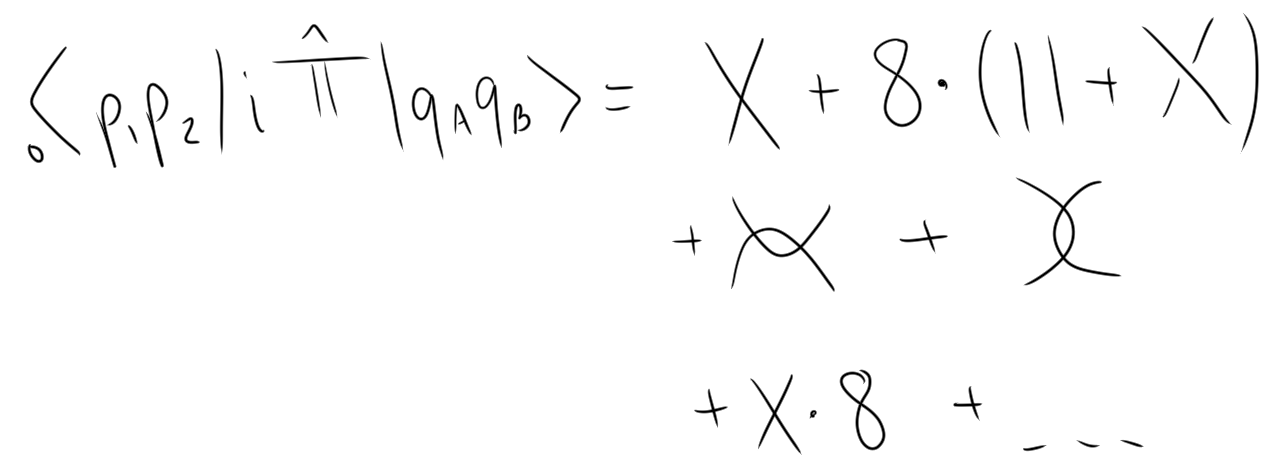
\includegraphics[scale=0.4]{images/tmatrix.png}
	\caption{Full diagrammatic expansion of the interacting component fo the $\mathcal{S}$-matrix.}
\end{figure}

\noindent These are the three types of diagrams, with respect to connectedness, that are always encountered: fully connected, partially connected, and vacuum bubble times cully connected.

\begin{figure}[H]
	\centering
	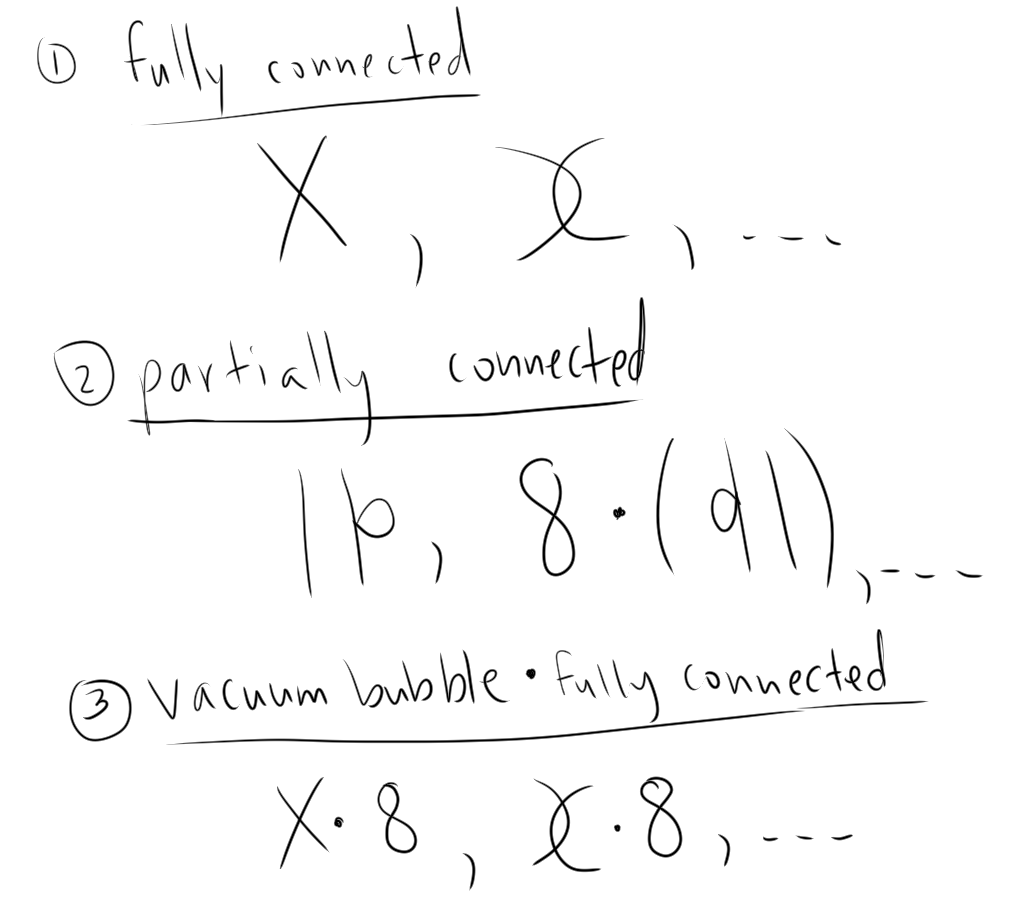
\includegraphics[scale=0.6]{images/connectiontypes.png}
	\caption{Three types of connectedness encountered in diagrammatic expansions of the interacting component of the $\mathcal{S}$-matrix.}
\end{figure}
 
\subsection*{Vacuum Bubbles and Fully Connected Diagrams}

\noindent Claim, here without proof, that products of vacuum bubbles and fully connected diagrams exponentiate, and, further, the only diagrams which contribute to the $\mathcal{S}$-matrix are the fully connected diagrams. There still exist fully connected diagrams (integrals) that result in infinities. To quell these infinities, either impose a cutoff scale, \textbf{or} argue that such a diagram does not contribute to the $\mathcal{S}$-matrix. \\

\begin{figure}[H]
	\centering
	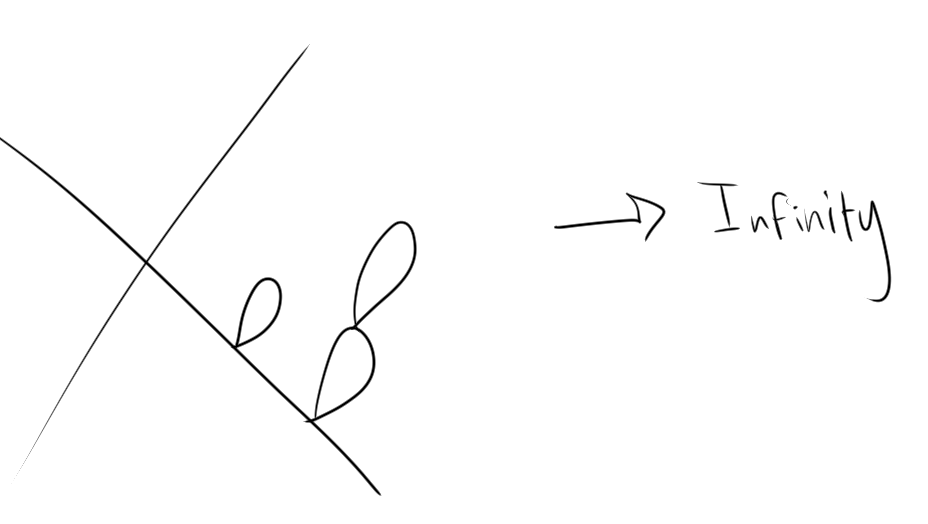
\includegraphics[scale=0.4]{images/fullconninf.png}
	\caption{An example of a fully connected diagram that results in infinity.}
\end{figure}

\noindent \textbf{External leg corrections} may be used to "amputate" parts of a diagram that will remove infinities from the external legs. This process represents a projection from the free momentum eigenstates to the interacting momentum eigenstates, just as in the projection of the vacuum state $\ket{\Omega}$. Thus, external leg corrections factorize the diagram. 
\begin{equation}
\ket{q_B}_0 \to \ket{q_B}
\end{equation}

\begin{figure}[H]
	\centering
	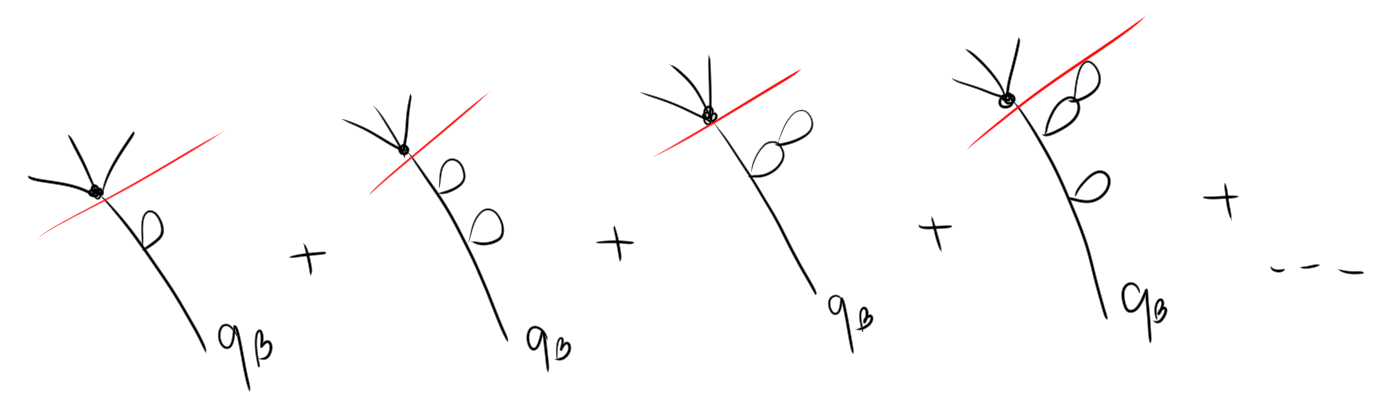
\includegraphics[scale=0.4]{images/extlegcorr.png}
	\caption{Single cuts made from the body of the diagram are called \textit{external leg corrections}, and "amputate" off infinities.}
\end{figure}

\noindent Amputation can not remove all infinities, since it is defined via the external leg corrections. Self-interactions on internal legs are not removable via amputation.

\begin{figure}[H]
	\centering
	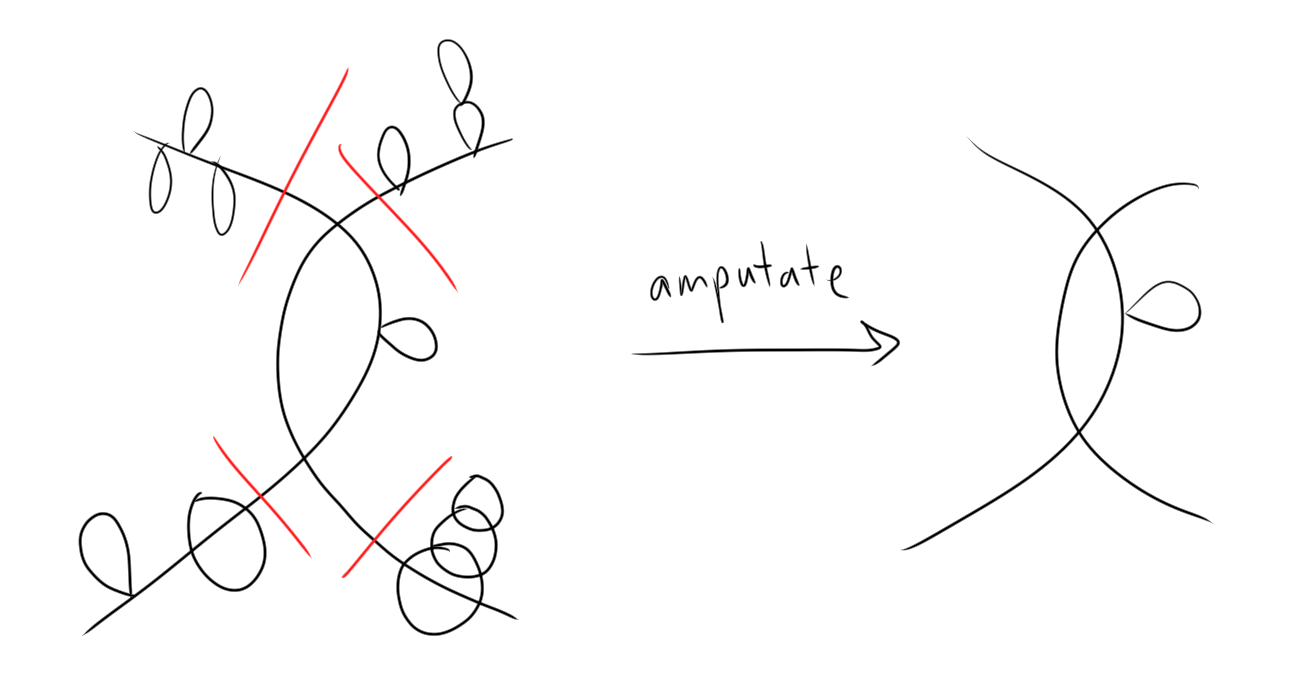
\includegraphics[scale=0.4]{images/amputation.png}
	\caption{An example of an amputation process where not all infinities can be removed, since it is not on an external leg.}
\end{figure}

\noindent And the final statement of the Feynman rule for the $\varphi^4$ interaction theory reads

\begin{equation}
i \mathcal{M} (2\pi)^4 \delta^{(4)} (q_A + q_B - \sum_f p_f) = \left( \stackanchor{\stackanchor{sum of all connected and}{amputated Feynamn diagrams}}{\stackanchor{with incoming momenta $q_A$, $q_B$}{and outgoing momenta $p_f$}} \right)
\end{equation}